   \begin{MyInnerSplitBox}{Year 8 and below}
      Four runners are at different positions around an athletics track. The track is divided into thirty sectors as indicated by the numbers round the periphery. Each runner moves forward the number of sectors indicated by the red arrow in front of them, in the same time. When they are next all in the same sector, which sector number will it be?
      \tcblower
        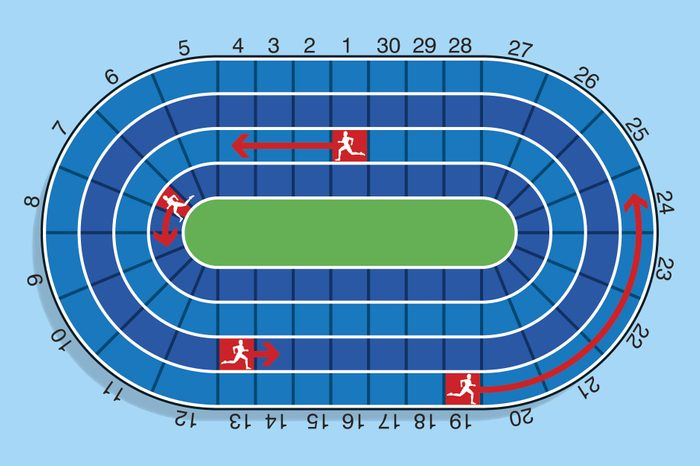
\includegraphics[width=\linewidth]{images/WP-track.jpg}
    \end{MyInnerSplitBox}
      \iftoggle{SOLUTION}{%conditional output begin
      \begin{MySolutionBox}
        Let's call the runner in sector 1 Runner 1, the runner in sector 7 Runner 2, the person in sector 13 Runner 3 and the athlete in sector 19 Runner 4.\par
        We don't know how long it takes Runner 1 to move from Sector 1 to Sector 4, but in that same time period, Runner 2 moves forward 2 sectors, Runner 3 moves on 1 sector and Runner 4 moves 5 sectors.\par
        We can write an expression for the sector number reached after \(t\) periods.\par
        \begin{tabular}{l|c|c|c|c|c}
          &Sector after& & & &\\
          &\(t\) periods& \(0\) & \(1\) & \(2\) & \(3\)\\ \hline
          Runner 1 & \(1+3t\) & \(1\) & \(4\) & \(7\) & \(10\)\\
          Runner 2 & \(7+2t\) & \(7\) & \(9\) & \(11\) & \(13\)\\
          Runner 3 & \(13+t\) & \(13\) & \(14\) & \(15\) & \(16\)\\
          Runner 4 & \(19+5t\) & \(19\) & \(24\) & \(29\) & \(4\)\\
        \end{tabular}\par\vspace{4mm}
      Notice that Runner 4's sector number 'wrapped round' to \(4\). \(29 + 5\) is \(34\) but they reached sector \(4\) on the track. This is arithmetic modulo 30, you have met the idea before with hours of the day. The hour after the \(24^{th}\) hour, isn't the \(25^{th}\) hour, it's the \(1^{st}\) hour (of the next day).\par
      We could just keep adding columns to our table until all the Runners' sector numbers became the same. This is a valid way of solving the problem, sometimes called a trial and error, or 'brute force' approach. The downside is that we often may have little idea of how many repetitions would be needed. Let's try to be a bit more analytical: We need to find the first value of \(t\) for which all runners are in the same sector.\par
      We need to find \(t\) for which the following is true:
       \begin{gather*}
          1 + 3t = 7 + 2t = 13 + t = 19 + 5t\\
          \shortintertext{we can subtract \(t\) throughout,}
          1 + 2t = 7 + t = 13 = 19 + 4t\\
          \shortintertext{and we can subtract \(1\) throughout,}
          2t = 6 + t = 12 = 18 + 4t
       \end{gather*}\par
       Taking equations pairwise from the last line, we have \(2t = 6+t\implies t=6\) and \(6+t=12\implies t=6\) and \(12=18+4t\). The first two give an answer of six time periods. Let's try that in our table:
         \begin{tabular}{l|c|c|c|c|c|c|c|c}
          &Sector after& & & & & & &\\
          &\(t\) periods& \(0\) & \(1\) & \(2\) & \(3\) & \(4\) & \(5\) & \(6\)\\ \hline
           Runner 1 & \(1+3t\) & \(1\) & \(4\) & \(7\) & \(10\) & \(13\) & \(16\) & \(19\)\\
           Runner 2 & \(7+2t\) & \(7\) & \(9\) & \(11\) & \(13\) & \(15\) & \(17\) & \(19\)\\
           Runner 3 & \(13+t\) & \(13\) & \(14\) & \(15\) & \(16\) & \(17\) & \(18\) & \(19\)\\
           Runner 4 & \(19+5t\) & \(19\) & \(24\) & \(29\) & \(4\) & \(9\) & \(14\) & \(19\)\\
        \end{tabular}\par\vspace{4mm}
        So we can see that \(t=6\) is a solution and the runners will be all together on sector 19 of the track after six time periods.\par
        But what about that last equation \(12=18+4t\) above? If we simplify: \(-6=4t\) and then substitute \(t=6\) into it we get \(-6=24\), which seems strange until we consider that we are counting modulo \(30\), six back from thirty is \(24\).\par
        \textbf{So Sector 19 is the answer.}
    \end{MySolutionBox}
      }{}%conditional output end



      % If we ignore the starting sectors of each runner for the moment, if they all started at the same point on the track, how many periods would it be before they are at the same place again? This is the equivalent to finding the least common multiple of \(1\), \(2\), \(3\) and \(5\), which is \(30\). In other words, after thirty time periods each runner would be back where they started.\par
      % Runner 1 would have gone three times round the track (\(3\times30\)),\par
      % Runner 2 would have gone twice round the track (\(2\times30\)),\par
      % Runner 3 would have gone once round the track (\(1\times30\)), and\par
      % Runner 4 would have gone five times round the track (\(5\times30\)).\par
      % Really, however, we want to find the first time they are all together in any sector, not necessarily the starting sector.

